\documentclass[12pt]{article}

% Use packages %
\usepackage{graphicx, courier, amsmath, amssymb, amscd, amsfonts, mathtools, bm, esint, leftidx, extarrows, latexsym, relsize, color, tikz, comment}
\usepackage[obeyspaces]{url}% http://ctan.org/pkg/url

% Set length %
\setlength{\textwidth}{160mm}
\setlength{\textheight}{235mm}
\setlength{\oddsidemargin}{-0mm}
\setlength{\topmargin}{-10mm}

% Define h-bar %
\newsavebox{\myhbar}
\savebox{\myhbar}{$\hbar$}
\renewcommand*{\hbar}{\mathalpha{\usebox{\myhbar}}}

% Chinese input %
%\usepackage{xeCJK} 
%\setCJKmainfont{微軟正黑體}
%\usepackage[T1]{fontenc}
%\makeatletter

% Equation number %
%\@addtoreset{equation}{section} 
%\renewcommand\theequation{{\thesection}.{\arabic{equation}}}
%\makeatletter 

% Helper Command %
\newcommand{\argmin}{\operatornamewithlimits{argmin}}
\newcommand{\rmnum}[1]{\romannumeral #1} 
\newcommand{\Rmnum}[1]{\expandafter\@slowromancap\romannumeral #1@}
\newcommand{\overbar}[1]{\mkern 1.5mu\overline{\mkern-1.5mu#1\mkern-1.5mu}\mkern 1.5mu}
\makeatother
\newcommand*{\QEDA}{\hfill\ensuremath{\blacksquare}}
\newcommand*{\QEDB}{\hfill\ensuremath{\square}}
\newcommand*{\BmVert}{\bigm\vert}
\newcommand{\bigslant}[2]{{\raisebox{.2em}{$#1$}\left/\raisebox{-.2em}{$#2$}\right.}}
\newcommand{\Nelements}[3]{\left\{ #1, ~ #2, \ldots, ~ #3 \right\}}
\newcommand{\CBrackets}[1]{\left\{#1\right\}}
\newcommand{\SBrackets}[1]{\left[#1\right]}
\newcommand{\ParTh}[1]{\left(#1\right)}
\newcommand{\Ceil}[1]{\left\lceil#1\right\rceil}
\newcommand{\Floor}[1]{\left\lfloor#1\right\rfloor}
\newcommand{\BF}[1]{{\bf#1}}
\newcommand{\Inverse}[1]{{#1}^{-1}}
\newcommand{\Generator}[1]{\left\langle#1\right\rangle}
\newcommand{\AbsVal}[1]{\left|#1\right|}
\newcommand{\VecAbsVal}[1]{\left\|#1\right\|}
\newcommand{\BSlash}[2]{\left.#1\middle\backslash#2\right.}
\newcommand{\Divide}[2]{\left.#1\middle/#2\right.}
\newcommand{\SciNum}[2]{#1\times{10}^{#2}}
\newcommand{\Matrix}[2]{\ParTh{\begin{array}{#1}#2\end{array}}}
\newcommand{\MatrixTwo}[4]{\ParTh{\begin{array}{cc}{#1}&{#2}\\{#3}&{#4}\end{array}}}
\newcommand{\MatrixNByN}[1]{\Matrix{cccc}{{#1}_{11} & {#1}_{12} & \cdots & {#1}_{1n} \\ {#1}_{21} & {#1}_{22} & \cdots & {#1}_{2n} \\ \vdots & \vdots & \ddots & \vdots \\ {#1}_{n1} & {#1}_{n2} & \cdots & {#1}_{nn}}}
\newcommand{\ndiv}{\hspace{-4pt}\not|\hspace{2pt}}
\newcommand{\eqdef}{\xlongequal{\text{def}}}%
\newcount\arrowcount
\newcommand\arrows[1]{\global\arrowcount#1 \ifnum\arrowcount>0
\begin{matrix}\expandafter\nextarrow\fi}
\newcommand\nextarrow[1]{\global\advance\arrowcount-1 \ifx\relax#1\relax\else \xrightarrow{#1}\fi\ifnum\arrowcount=0 \end{matrix}\else\\\expandafter\nextarrow\fi}
\newcommand{\horrule}[1]{\rule{\linewidth}{#1}}

% Tikz settings %
\usetikzlibrary{shapes,arrows}
\tikzstyle{decision} = [diamond, draw, fill=white!20, text width=4.5em, text badly centered, node distance=3cm, inner sep=0pt]
\tikzstyle{block}    = [rectangle, draw, fill=white!20, text width=8em, text centered, rounded corners, minimum height=4em]
\tikzstyle{point}    = [fill = white!20, minimum size=0.5cm]
\tikzstyle{line}     = [draw, -latex']
\tikzstyle{mapsto}   = [draw, |->]
\tikzstyle{cloud}    = [draw, ellipse,fill=red!20, node distance=3cm, minimum height=2em]
%%%%%%%%%%%%%%%%%%%%%%%%%%%%%%%%%%%%%%%%%%%%%%%%%%%%%%%%%%%%%%%%%%%%%%%%%%%%%%%%%%%%%%%%%%%%%%%%%%%%%%%%%%%%%%%%%%
%%%%%%%%%%%%%%%%%%%%%%%%%%%%%%%%%%%%%%%%%%%%%%%%%%%%%%%%%%%%%%%%%%%%%%%%%%%%%%%%%%%%%%%%%%%%%%%%%%%%%%%%%%%%%%%%%%

\begin{document}
%%%%%%%%%%%%%%%%%%%%%%%%%%%%%%%%%%%%%%%%%%%%%%%%%%%%%%%%%%%%%%%%%%%%%%%%%%%%%%%%%%%%%%%%%%%%%%%%%%%%%%%%%%%%%%%%%%%%%%%%%%%%%%%%%%%%%%%%%%%%%%%%%%%%%%%%%%%
%%%%%%%%%%%%%%%%%%%%%%%%%%%%%%%%%%%%%%%%%%%%%%%%%%%%%%%%%%%%%%%%%%%%%%%%%%%%%%%%%%%%%%%%%%%%%%%%%%%%%%%%%%%%%%%%%%%%%%%%%%%%%%%%%%%%%%%%%%%%%%%%%%%%%%%%%%%
\baselineskip 6.5mm
\setlength{\parindent}{0pt}
\title{ 
\normalfont \normalsize 
\horrule{0.5pt} \\[0.4cm]
\huge { \Huge Machine Learning \\ \large Answer Sheet for Homework 1 }\\ % The assignment title
\horrule{2pt} \\ [0.5cm]
}
\author{ { \Large Da-Min HUANG } \\
{\small R04942045} \\
{\small\textit{Graduate Institute of Communication Engineering, National Taiwan University}}
}
\date{October 14, 2015}
\allowdisplaybreaks[4]
\maketitle
%%%%%%%%%%%%%%%%%%%%%%%%%%%%%%%%%%%%%%%%%%%%%%%%%%%%%%%%%%%%%%%%%%%%%%%%%%%%%%%%%%%%%%%%%%%%%%%%%%%%%%%%%%%%%%%%%%
%%%%%%%%%%%%%%%%%%%%%%%%%%%%%%%%%%%%%%%%%%%%%%%%%%%%%%%%%%%%%%%%%%%%%%%%%%%%%%%%%%%%%%%%%%%%%%%%%%%%%%%%%%%%%%%%%%

\subsection*{Problem 1}

\begin{enumerate}

\item[(\rmnum{1})] Prime number has its math and programmable definition.

\item[(\rmnum{2})]
\begin{enumerate}
\item[$\bullet$] Pattern: how the credit card charged.
\item[$\bullet$] Definition: not easily programmable.
\item[$\bullet$] Data: history of bank operation.
\end{enumerate}

\item[(\rmnum{3})] It has programmable definition.

\item[(\rmnum{4})]
\begin{enumerate}
\item[$\bullet$] Pattern: cycle for traffic lights.
\item[$\bullet$] Definition: not easily programmable.
\item[$\bullet$] Data: history of traffic condition.
\end{enumerate}

\item[(\rmnum{5})]
\begin{enumerate}
\item[$\bullet$] Pattern: age of people.
\item[$\bullet$] Definition: not enough data.
\item[$\bullet$] Data: medical record.
\end{enumerate}

\end{enumerate}
Hence, the answer is (\rmnum{2}), (\rmnum{4}) and (\rmnum{5}).

\QEDB

\horrule{0.5pt}

\subsection*{Problem 2}

It learns with implicit information sequentially so it is type of reinforcement learning.

\QEDB

\horrule{0.5pt}

\subsection*{Problem 3}

It learns without labels so it is type of unsupervised learning.

\QEDB

\horrule{0.5pt}

\subsection*{Problem 4}

Every picture has its label (face or non-face) so it is type of supervised learning.

\QEDB

\horrule{0.5pt}

\subsection*{Problem 5}

It schedule experiments strategically so it is type of active learning.

\QEDB

\horrule{0.5pt}

\subsection*{Problem 6}

Now we have
\begin{align}
E_{OTS}\ParTh{g,~f}=\dfrac{1}{L}\sum_{\ell=1}^{L}\SBrackets{g\ParTh{\BF{x_{N+\ell}}}\neq f\ParTh{\BF{x}_{N+\ell}}}
\end{align}
It is easily to find that $g\ParTh{\BF{x_{N+\ell}}}\neq f\ParTh{\BF{x}_{N+\ell}}$ when $N+\ell$ is even. So
\begin{align}
\sum_{\ell=1}^{L}\SBrackets{g\ParTh{\BF{x_{N+\ell}}}\neq f\ParTh{\BF{x}_{N+\ell}}}=\left\lfloor\dfrac{N+L}{2}\right\rfloor-\Floor{\dfrac{L}{2}}
\end{align}
since there are $\Floor{\Divide{z}{2}}$ even numbers between $1$ and $z\in\mathbb{Z}$. Hence,
\begin{align}
E_{OTS}\ParTh{g,~f}=\dfrac{1}{L}\ParTh{\left\lfloor\dfrac{N+L}{2}\right\rfloor-\Floor{\dfrac{L}{2}}}
\end{align}

\QEDB

\horrule{0.5pt}

\subsection*{Problem 7}

Since $f$ generate $\mathcal{D}$ so the output of $f$ is fixed for $1\leq n\leq N$.

There are still $L$ terms need to be determined, each with two choices ($-1$ or $+1$). So the answer is $2^L$.

\QEDB

\horrule{0.5pt}

\subsection*{Problem 8}

\begin{comment}
Since $\mathcal{A}_1$ and $\mathcal{A}_2$ generate $\mathcal{D}$ in a noiseless setting, so
\begin{align}
\CBrackets{E_{OTS}\ParTh{\mathcal{A}_1,~f}}^N_{n=1}=\CBrackets{E_{OTS}\ParTh{\mathcal{A}_2,~f}}^N_{n=1}=\CBrackets{0}
\end{align}
But for $N<n\leq N+L$,
\begin{align}
\mathbb{P}_f\CBrackets{\CBrackets{E_{OTS}\ParTh{\mathcal{A}_1,~f}}^{N+L}_{n=N+1}=\CBrackets{E_{OTS}\ParTh{\mathcal{A}_2,~f}}^{N+L}_{n=N+1}}=\dfrac{1}{2^L}
\end{align}
\end{comment}
If all those $f$ that can generate $\mathcal{D}$ in a noiseless setting are equally likely in probability, from previous problem, we know that there are $2^L$ possible $f$.

Thus, for $\BF{x}=\BF{x}_k$, $N+1\leq k\leq N+L$, $f\ParTh{\BF{x}_k}=+1\text{ or }-1$.

So
\begin{align}
\mathbb{E}_f\CBrackets{E_{OTS}\ParTh{g,~f}}&=\mathbb{E}_f\ParTh{\dfrac{1}{L}\sum_{\ell=1}^{L}\SBrackets{g\ParTh{\BF{x_{N+\ell}}}\neq f\ParTh{\BF{x}_{N+\ell}}}}
\\
&=\dfrac{1}{L}\mathbb{E}_f\ParTh{\sum_{\ell=1}^{L}\SBrackets{g\ParTh{\BF{x_{N+\ell}}}\neq f\ParTh{\BF{x}_{N+\ell}}}}\\
&=\dfrac{1}{L}\ParTh{\underbrace{\dfrac{L}{2}}_{\text{Expected error number}}}=\dfrac{1}{2}
\end{align}
Since $\mathcal{A}_1$ and $\mathcal{A}_2$ are deterministic, we have
\begin{align}
\mathbb{E}_f\CBrackets{E_{OTS}\ParTh{g,~f}}=\mathbb{E}_f\CBrackets{E_{OTS}\ParTh{\mathcal{A}_1,~f}}=\mathbb{E}_f\CBrackets{E_{OTS}\ParTh{\mathcal{A}_2,~f}}
\end{align}
\begin{comment}
and
\begin{align}
\mathbb{E}_f\CBrackets{E_{OTS}\ParTh{\mathcal{A}_2,~f}}&=\mathbb{E}_f\ParTh{\dfrac{1}{L}\sum_{\ell=1}^{L}\SBrackets{\mathcal{A}_2\ParTh{\BF{x_{N+\ell}}}\neq f\ParTh{\BF{x}_{N+\ell}}}}
\\
&=\dfrac{1}{L}\mathbb{E}_f\ParTh{\sum_{\ell=1}^{L}\SBrackets{\mathcal{A}_2\ParTh{\BF{x_{N+\ell}}}\neq f\ParTh{\BF{x}_{N+\ell}}}}\\
&=\dfrac{1}{L}\ParTh{\dfrac{L}{2}}=\dfrac{1}{2}
\end{align}
because there are only 2 output choices, so the expectation value of error rate should be $\Divide{1}{2}$ in a noiseless setting.
%\mathbb{E}_f\CBrackets{E_{OTS}\ParTh{\mathcal{A}_2,~f}}
\end{comment}

\QEDB

\horrule{0.5pt}

\subsection*{Problem 9}

If $\nu = 0.5$, then there are 5 orange marbles.
\begin{align}
\mathbb{P}\ParTh{\text{5 orange marbles}}=\underbrace{\ParTh{0.5}^5}_{\text{5 orange}}\times\underbrace{\ParTh{0.5}^5}_{\text{5 green}}\times\binom{10}{5}=\dfrac{63}{256}\approx0.2461
\end{align}

\QEDB

\horrule{0.5pt}

\subsection*{Problem 10}

If $\nu = 0.9$, then there are 9 orange marbles.
\begin{align}
\mathbb{P}\ParTh{\text{9 orange marbles}}=\underbrace{\ParTh{0.9}^9}_{\text{9 orange}}\times\underbrace{\ParTh{0.1}^1}_{\text{1 green}}\times\binom{10}{9}=\dfrac{3^{18}}{2^9\times5^9}\approx0.3874
\end{align}

\QEDB

\horrule{0.5pt}

\subsection*{Problem 11}

If $\nu \leq 0.1$, then there are 1 orange marbles or 0 orange marbles,
\begin{align}
\mathbb{P}\ParTh{\text{1 orange marbles}}&=\underbrace{\ParTh{0.9}^1}_{\text{1 orange}}\times\underbrace{\ParTh{0.1}^9}_{\text{9 green}}\times\binom{10}{1}=\SciNum{9.0}{-9}\\
\mathbb{P}\ParTh{\text{0 orange marbles}}&=\underbrace{\ParTh{0.1}^{10}}_{\text{10 green}}=\SciNum{0.1}{-9}\\
\Rightarrow\mathbb{P}\ParTh{\nu\leq0.1}&=\SciNum{9.0}{-9}+\SciNum{0.1}{-9}=\SciNum{9.1}{-9}
\end{align}

\QEDB

\horrule{0.5pt}

\subsection*{Problem 12}

By Hoeffding's Inequality: $\mathbb{P}\SBrackets{\AbsVal{\nu-\mu}>\epsilon}\leq2\exp\ParTh{-2\epsilon^2N}$, we have
\begin{align}
\text{Bound}=2\exp\ParTh{-2\times\ParTh{0.9-0.1}^2\times10}=\SciNum{5.52}{-6}
\end{align}

\QEDB

\horrule{0.5pt}

\subsection*{Problem 13}

To get all orange 1, we can only pick B or C kind. Since each kind is with same quantity, then we have
\begin{align}
\mathbb{P}\ParTh{\text{pick B or C}}=\dfrac{1}{2}
\end{align}
so
\begin{align}
\mathbb{P}\ParTh{\text{all orange 1}}=\dfrac{1}{2}^5=\dfrac{1}{32}=\dfrac{8}{256}
\end{align}

\QEDB

\horrule{0.5pt}

\subsection*{Problem 14}

Consider the situations:
\begin{enumerate}
\item Only one number purely orange.

The only possible number are 2 and 5. So
\begin{align}
\mathbb{P}\ParTh{\text{only 2}}=\dfrac{1}{4^5}\ParTh{\underbrace{\binom{5}{1}}_{\text{1A4C}}+\underbrace{\binom{5}{2}}_{\text{2A3C}}+\underbrace{\binom{5}{3}}_{\text{3A2C}}+\underbrace{\binom{5}{4}}_{\text{4A1C}}}=\dfrac{30}{1024}=\mathbb{P}\ParTh{\text{only 5}}
\end{align}
\item Two numbers purely orange.

The possible numbers pair are $\ParTh{1,~3}$ and $\ParTh{4,~6}$. So
\begin{align}
\mathbb{P}\ParTh{\ParTh{1,~3}}=\dfrac{1}{4^5}\ParTh{\underbrace{\binom{5}{1}}_{\text{1B4C}}+\underbrace{\binom{5}{2}}_{\text{2B3C}}+\underbrace{\binom{5}{3}}_{\text{3B2C}}+\underbrace{\binom{5}{4}}_{\text{4B1C}}}=\dfrac{30}{1024}=\mathbb{P}\ParTh{\ParTh{4,~6}}
\end{align}
\item Three numbers purely orange.

The possible numbers pair are $\ParTh{1,~2,~3}$, $\ParTh{4,~5,~6}$, $\ParTh{1,~3,~5}$ and $\ParTh{2,~4,~6}$. So
\begin{align}
\mathbb{P}\ParTh{\ParTh{1,~2,~3}}=\dfrac{1}{4^5}=\dfrac{1}{1024}=\mathbb{P}\ParTh{\ParTh{4,~5,~6}}=\mathbb{P}\ParTh{\ParTh{1,~3,~5}}=\mathbb{P}\ParTh{\ParTh{2,~4,~6}}
\end{align}
\end{enumerate}
So
\begin{align}
\mathbb{P}\ParTh{\text{some number purely orange}}=2\times\dfrac{30}{1024}+2\times\dfrac{30}{1024}+4\times\dfrac{1}{1024}=\dfrac{31}{256}
\end{align}

\QEDB

\horrule{0.5pt}

\subsection*{Problem 15}

The number of updates before the
algorithm halts is 45 times update, the index of the example that results in the last mistake is 135.

\QEDB

\horrule{0.5pt}

\subsection*{Problem 16}

The average number of updates before the
algorithm halts is 40.477. And the histogram is
\begin{figure}[h]
\centering
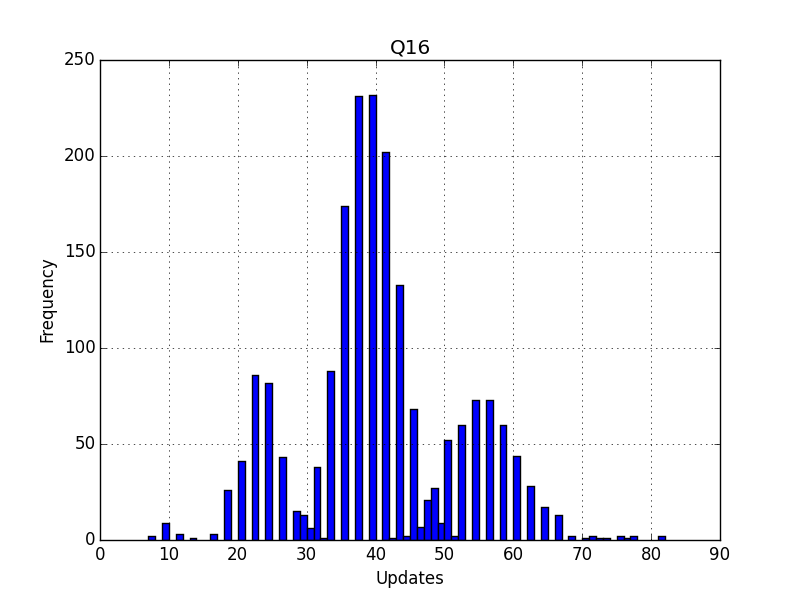
\includegraphics[scale=0.3]{Q16}
\caption{Q16 histogram}
\label{Q16}
\end{figure}

\QEDB

\horrule{0.5pt}

\subsection*{Problem 17}

The average number
of updates before the algorithm halts 40.219.
\begin{figure}[h]
\centering
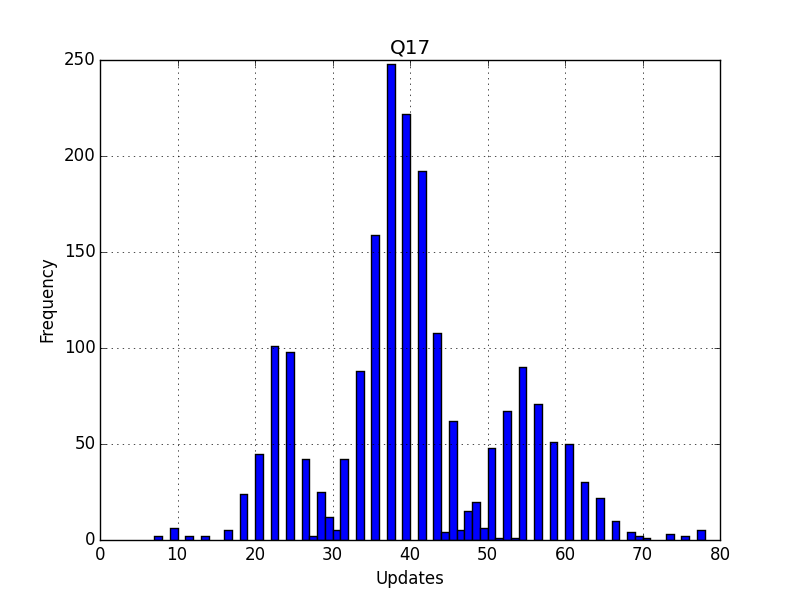
\includegraphics[scale=0.2]{Q17}
\caption{Q17 histogram}
\label{Q17}
\end{figure}
Compare with the previous problem, we can see that they are similar. But the peak of $\eta=0.5$ moves a little left. Test for $\eta=0.1$ and $\eta=0.01$, we have
\newpage
\begin{figure}[h]
\centering
  \begin{minipage}[b]{0.45\textwidth}
    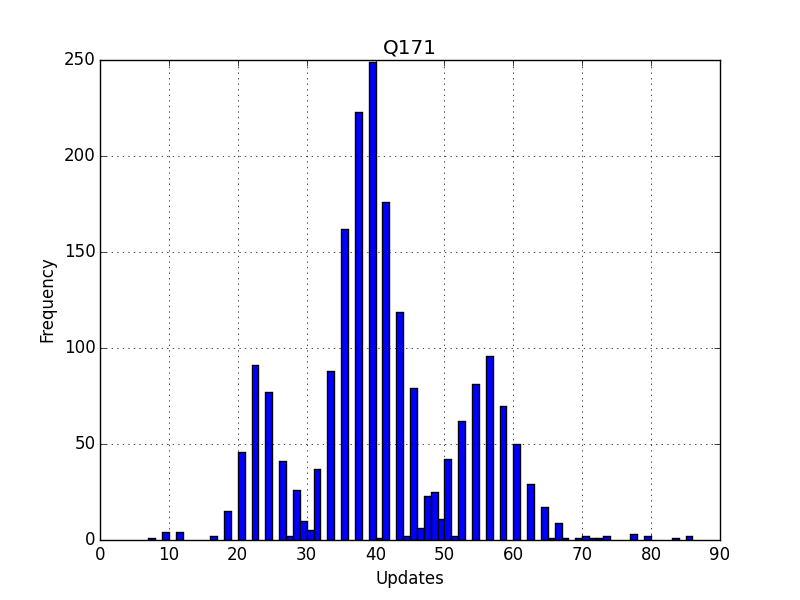
\includegraphics[width=\textwidth]{Q171.png}
    \caption{Q17 with $\eta=0.1$}
  \end{minipage}
  \hfill
  \begin{minipage}[b]{0.45\textwidth}
    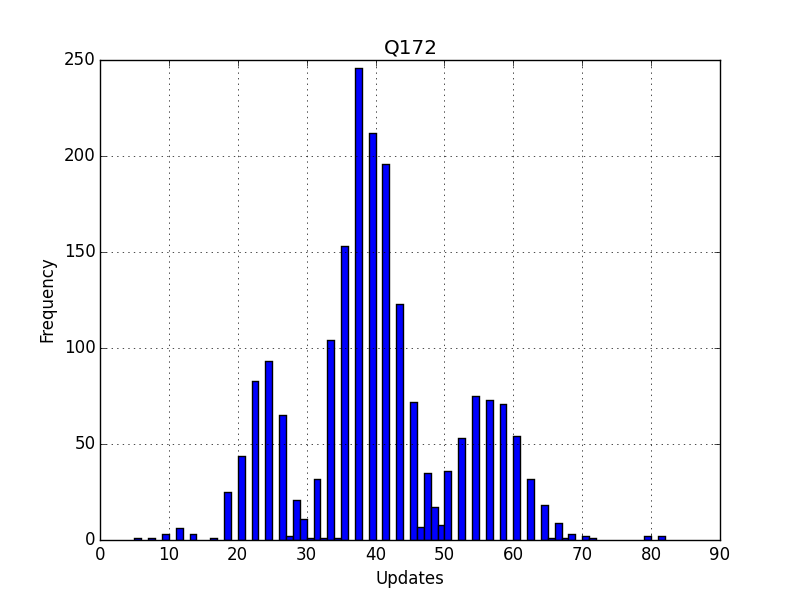
\includegraphics[width=\textwidth]{Q172.png}
    \caption{Q17 with $\eta=0.01$}
  \end{minipage}
\end{figure}
Seems like have no trend of moving left and the average is still around 40 (39.97 and 39.982, respectively). So the value of $\eta$ affects the number of updates little.

In fact, this because initial value of $\BF{w}$ is $\BF{0}$. So even the update term $\eta y_{n\ParTh{t}}\BF{x}_{n\ParTh{t}}$ is small, we still have
\begin{align}
\dfrac{\VecAbsVal{\BF{w}_{\eta=0.5}}}{\VecAbsVal{\BF{w}}}=\eta, ~ \dfrac{\BF{w}_{\eta=0.5}}{\VecAbsVal{\BF{w}_{\eta=0.5}}}\cdot\dfrac{\BF{w}}{\VecAbsVal{\BF{w}}}=1
\end{align}
This implies $\eta$ only affects the absolute value of $\BF{w}_\eta$. So the number of update will not change.

\QEDB

\horrule{0.5pt}
\newpage
\subsection*{Problem 18}

The average error rate on the test set is 0.130997.
\begin{figure}[h]
\centering
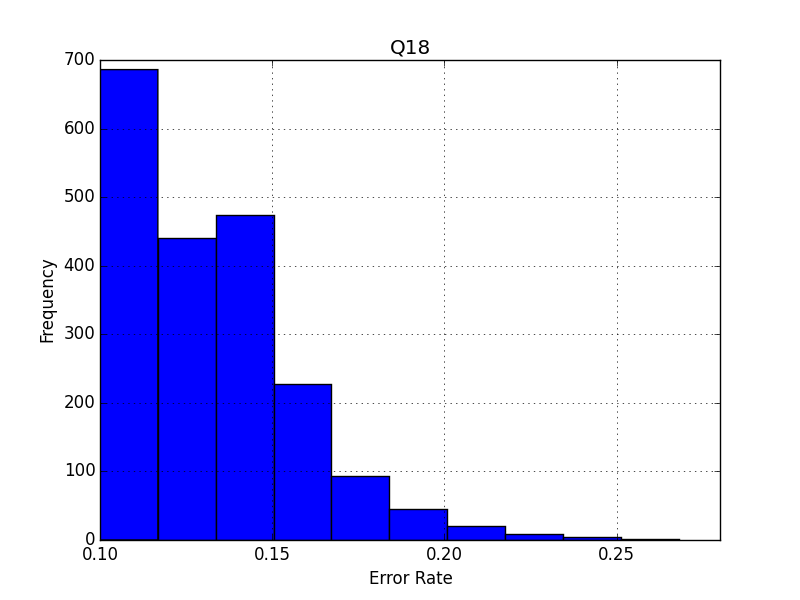
\includegraphics[scale=0.3]{Q18}
\caption{Q18 histogram}
\label{Q18}
\end{figure}

\QEDB

\horrule{0.5pt}

\subsection*{Problem 19}

The average error rate on the test set is 0.364533.
\begin{figure}[h]
\centering
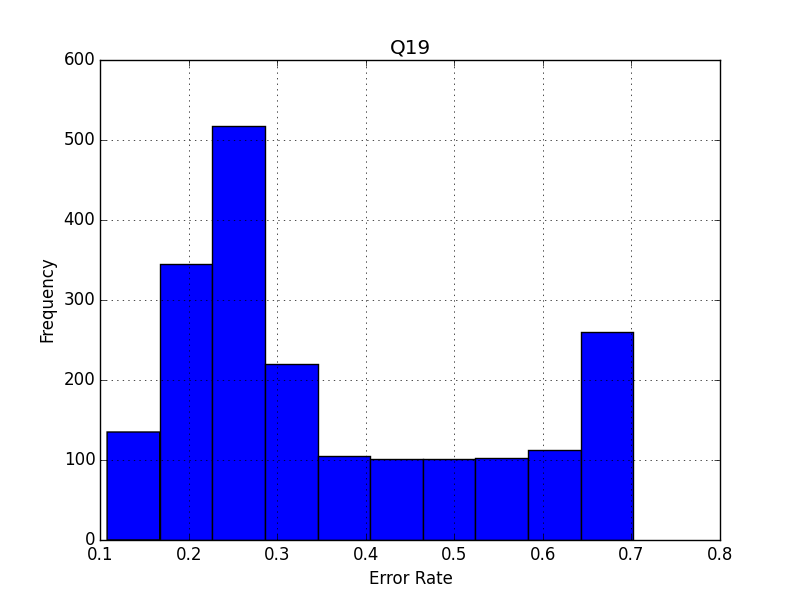
\includegraphics[scale=0.3]{Q19}
\caption{Q19 histogram}
\label{Q19}
\end{figure}
Compare with previous problem, we see that the error rate is not monotonic decreasing, with two local maximum around 0.3 and 0.7. Distribution of error rate is irregular.

\QEDB

\horrule{0.5pt}

\subsection*{Problem 20}

The average error rate on the test set is 0.11408.
\begin{figure}[h]
\centering
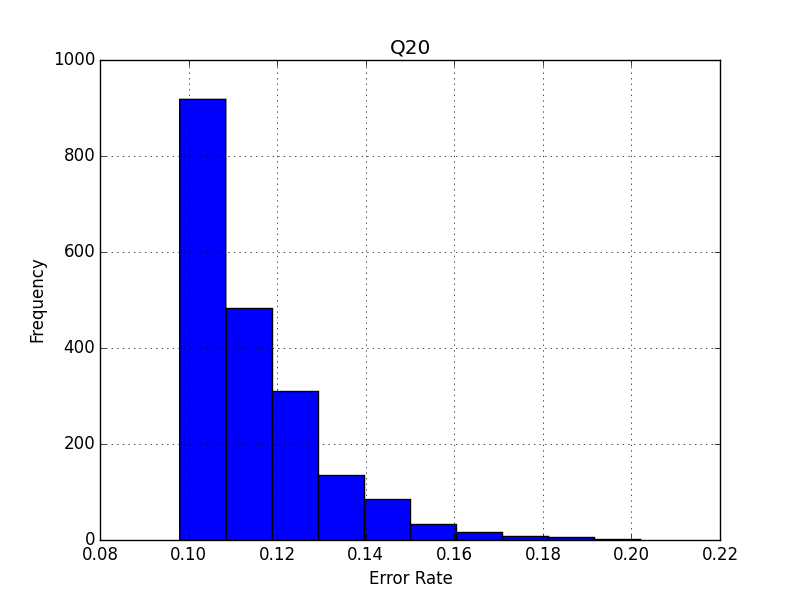
\includegraphics[scale=0.3]{Q20}
\caption{Q20 histogram}
\label{Q20}
\end{figure}

Compare with Problem 18, the figure is still monotonic decreasing. But the number between error rate$=0.10$ and $0.11$ increases, about 1.1 $\sim$ 1.5 times greater than Q18's. So the increase number of updates lower the average of error rate.

\QEDB

\horrule{0.5pt}

\subsection*{Problem 21}

Use python to calculate the time factor,
\begin{figure}[h]
\centering
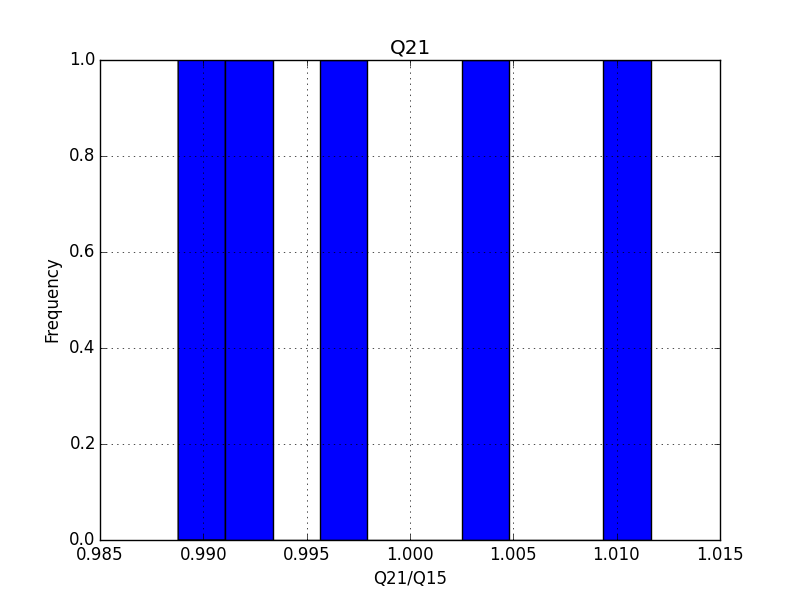
\includegraphics[scale=0.3]{Q21}
\caption{Q21 histogram}
\label{Q21}
\end{figure}

where
\begin{align}
\Divide{\text{Q21}}{\text{Q15}}=\dfrac{\text{Time of PLA as all }\BF{x}_n\text{(train set of Q15) scale down by a factor of 20}}{\text{Time of normal PLA}}
\end{align}
The histogram record $\Divide{\text{Q21}}{\text{Q15}}$ in repeated 20 times. We can find that two methods costs almost same time. Since we scale down all $\BF{x}_n$, so during every update of $\BF{w}_t$,
\begin{align}
\BF{w}_{t+1}\leftarrow\BF{w}_t+y_{n\ParTh{t}}\ParTh{\Divide{\BF{x}_{n\ParTh{t}}}{20}}=\BF{w}_t+\dfrac{1}{20}y_{n\ParTh{t}}{{\BF{x}_{n\ParTh{t}}}}
\end{align}
From the conclusion of Problem 17, we know that the factor acts just like $\eta$, so it does not make PLA algorithm run faster if the initial value of $\BF{w}$ is $\BF{0}$.

Also, if the initial value of $\BF{w}$ is not $\BF{0}$, it should cost more time to update the angle of $\BF{w}$ to final result since the update term is smaller.

\QEDB

\horrule{0.5pt}

\section*{Reference}

\begin{enumerate}

\item[{[1]}] Lecture Notes by Hsuan-Tien LIN, Department of Computer Science and Information Engineering, National Taiwan University, Taipei 106, Taiwan.

\end{enumerate}

%%%%%%%%%%%%%%%%%%%%%%%%%%%%%%%%%%%%%%%%%%%%%%%%%%%%%%%%%%%%%%%%%%%%%%%%%%%%%%%%%%%%%%%%%%%%%%%%%%%%%%%%%%%%%%%%%%%%%%%%%%%%%%%%%%%%%%%%%%%%%%%%%%%%%%%%%%%
%%%%%%%%%%%%%%%%%%%%%%%%%%%%%%%%%%%%%%%%%%%%%%%%%%%%%%%%%%%%%%%%%%%%%%%%%%%%%%%%%%%%%%%%%%%%%%%%%%%%%%%%%%%%%%%%%%%%%%%%%%%%%%%%%%%%%%%%%%%%%%%%%%%%%%%%%%%
\end{document}